\section{Expedition Findings}

The initial effort of the expedition was directed into setting up underground camp.

    \begin{marginfigure}
\checkoddpage \ifoddpage \forcerectofloat \else \forceversofloat \fi
\centering
 \frame{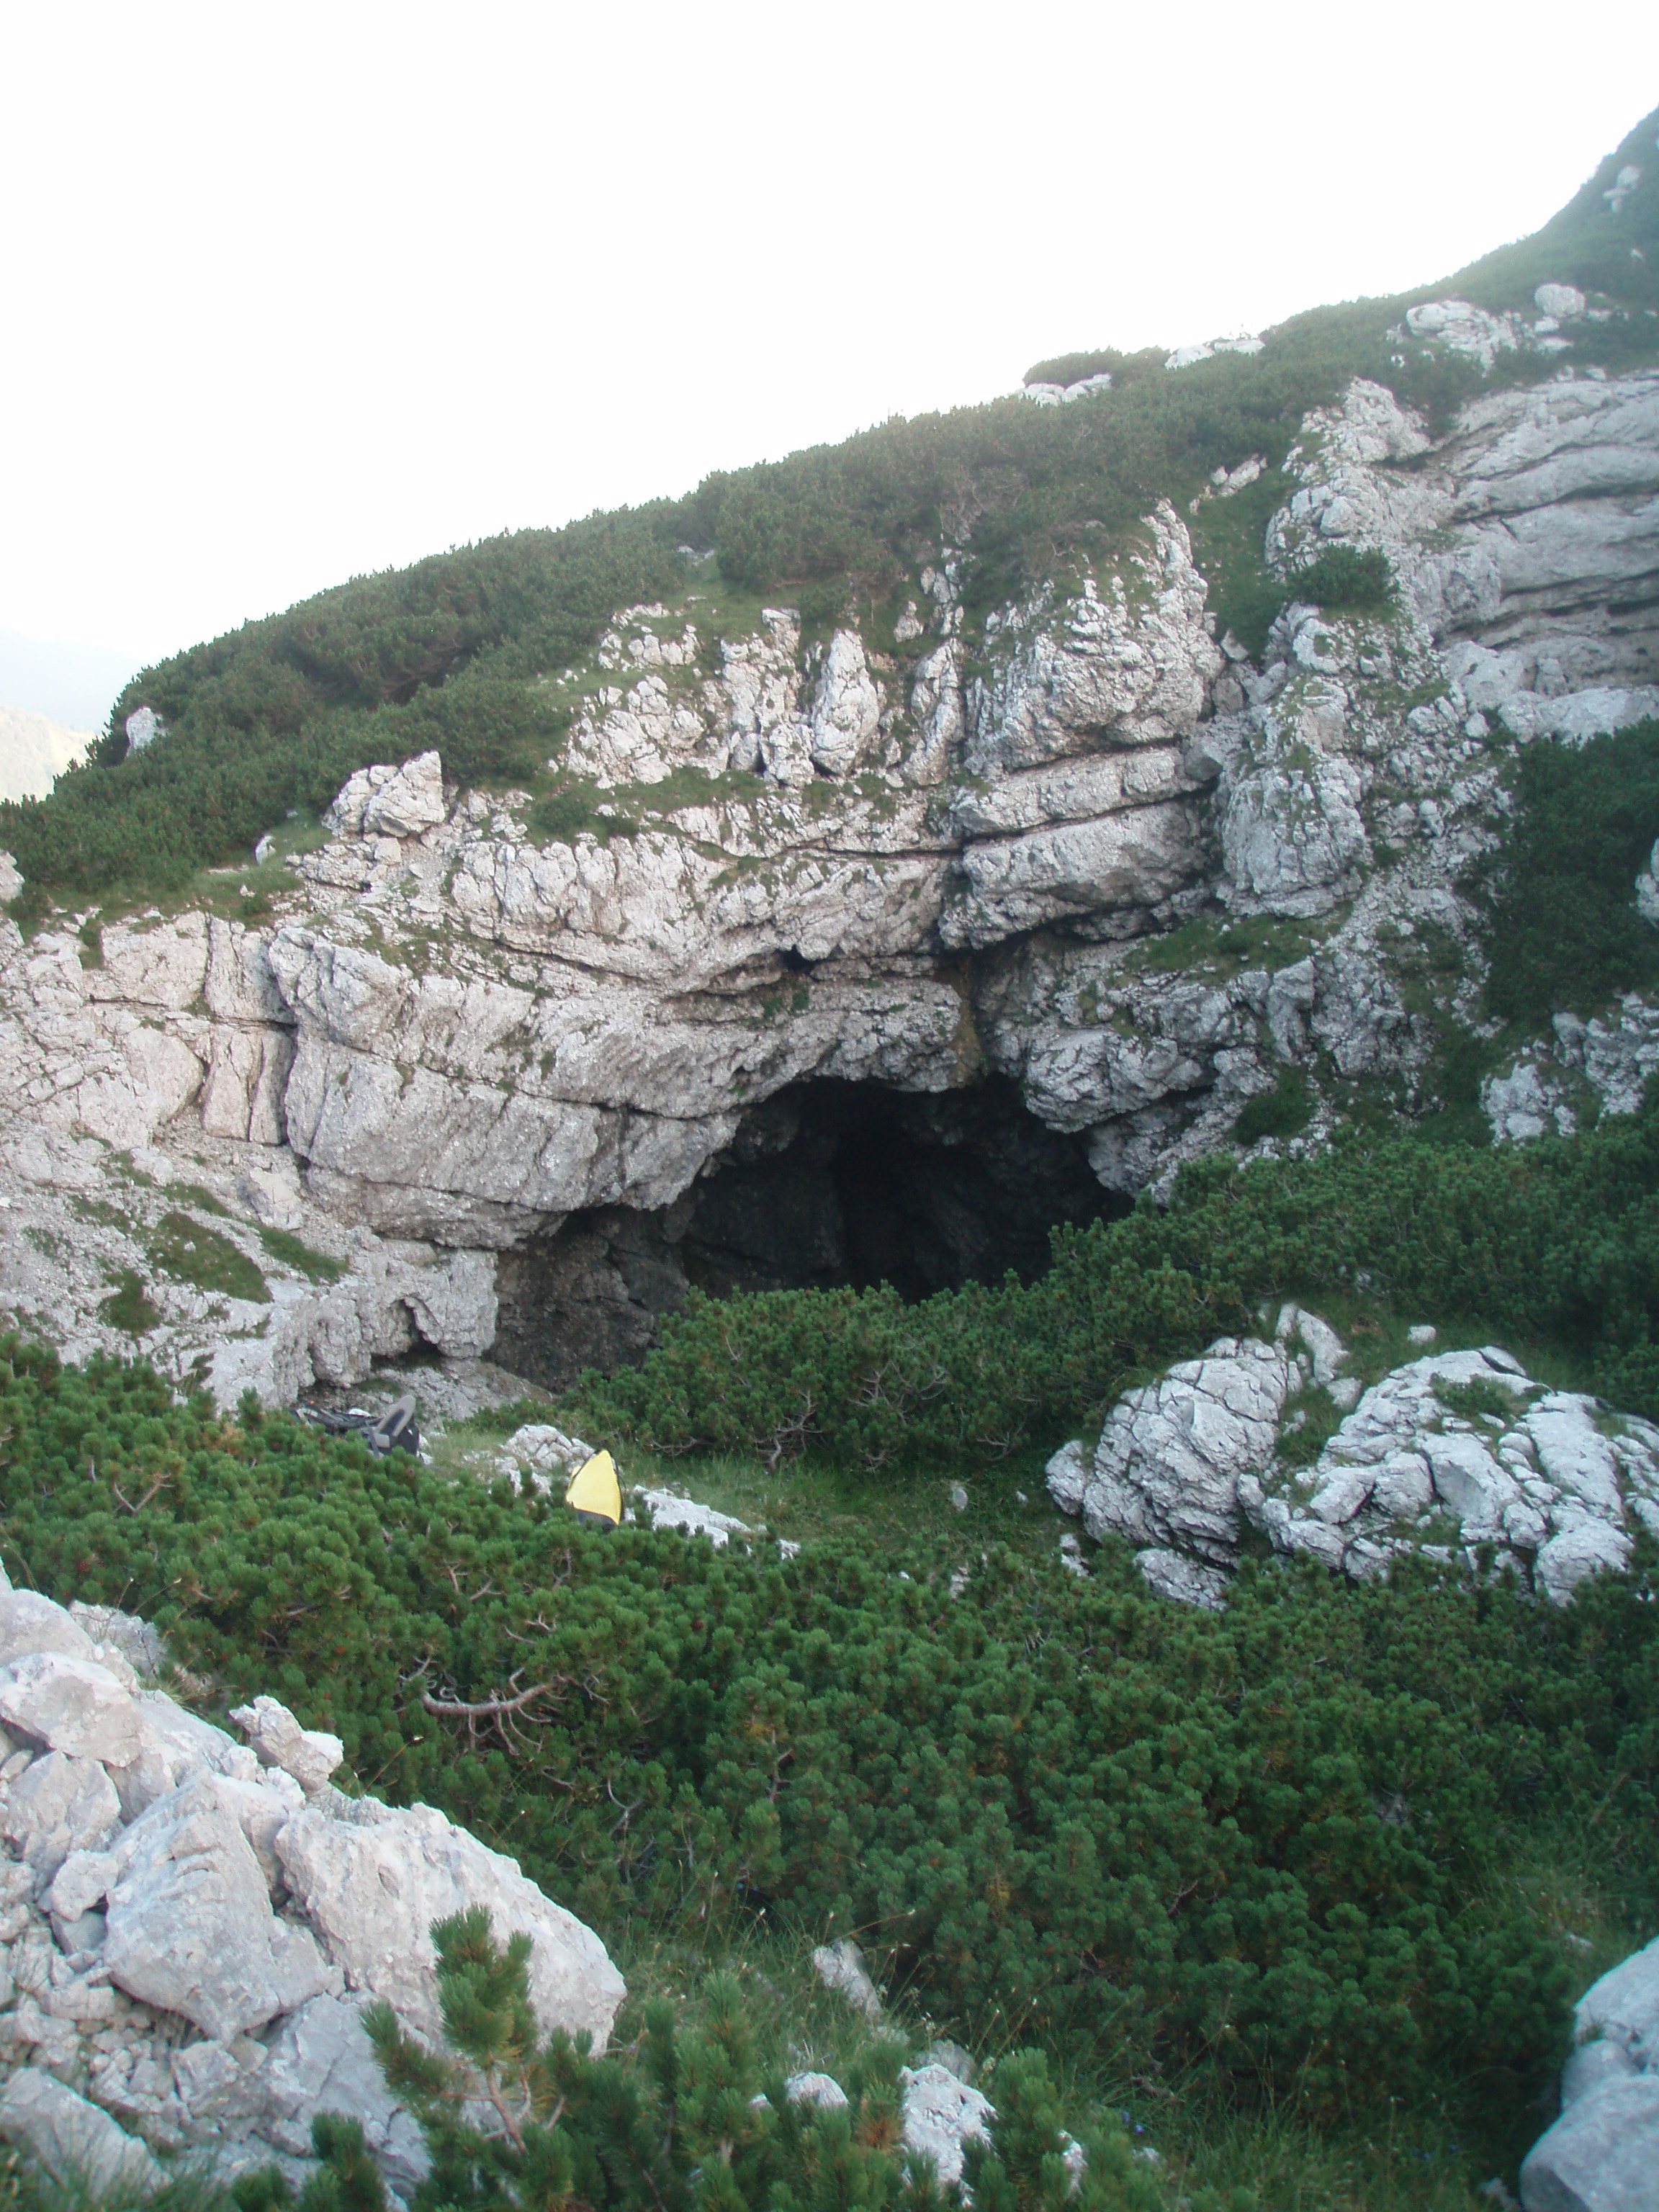
\includegraphics[width=\linewidth]{2010/expo_findings/20100809-05-35-44 - Jan Evetts - P2090134 - valley on plateau east of migovec--orig.jpg}} 
 \caption{Surface exploration went on in 2010 as always, such as in a valley on the plateau east of \passage[mountain]{Migovec}. \pic{Jan Evetts}}
 \label{valley east of Mig}
\end{marginfigure}

As the first pushing trips from this underground camp came back with
positive news, exploration based from camp (i.e. deep in \passage{Vrtnarija}) quickly became the main focus of expedition effort.

This came at the cost of further work in bounce trips down \passage{Captain Kangaroo} (the likely connection region to \passage{M2}) and \passage{M2} / \passage{SysMig} itself.

The usual surface bashing continued, looking for new cave systems on the
plateau. A revisit was made to the area north of \passage[mountain]{Kuk} (\passage{Area N}). This region is
heavily cratered with clear cave development, but the fear is that the
limestone is too broken and chossy for a human sized entrance.

We first visited this region with a serious aim of cave exploration in
2008, and returned in December 2009 on a `winter recce' by a two person
team with ice axe and crampons to identify which surface features were
actively linked into extensive underground systems through the holes
blown in the snow. Several more entrances were identified during this
recce, ones that were likely to be continued to be ignored in the summer
due to their unusual position.

These entrances were relocated (by GPS) this summer, but no new descents were made.


\subsection{Leopard}

\begin{marginfigure}
\checkoddpage \ifoddpage \forcerectofloat \else \forceversofloat \fi
\centering
 \frame{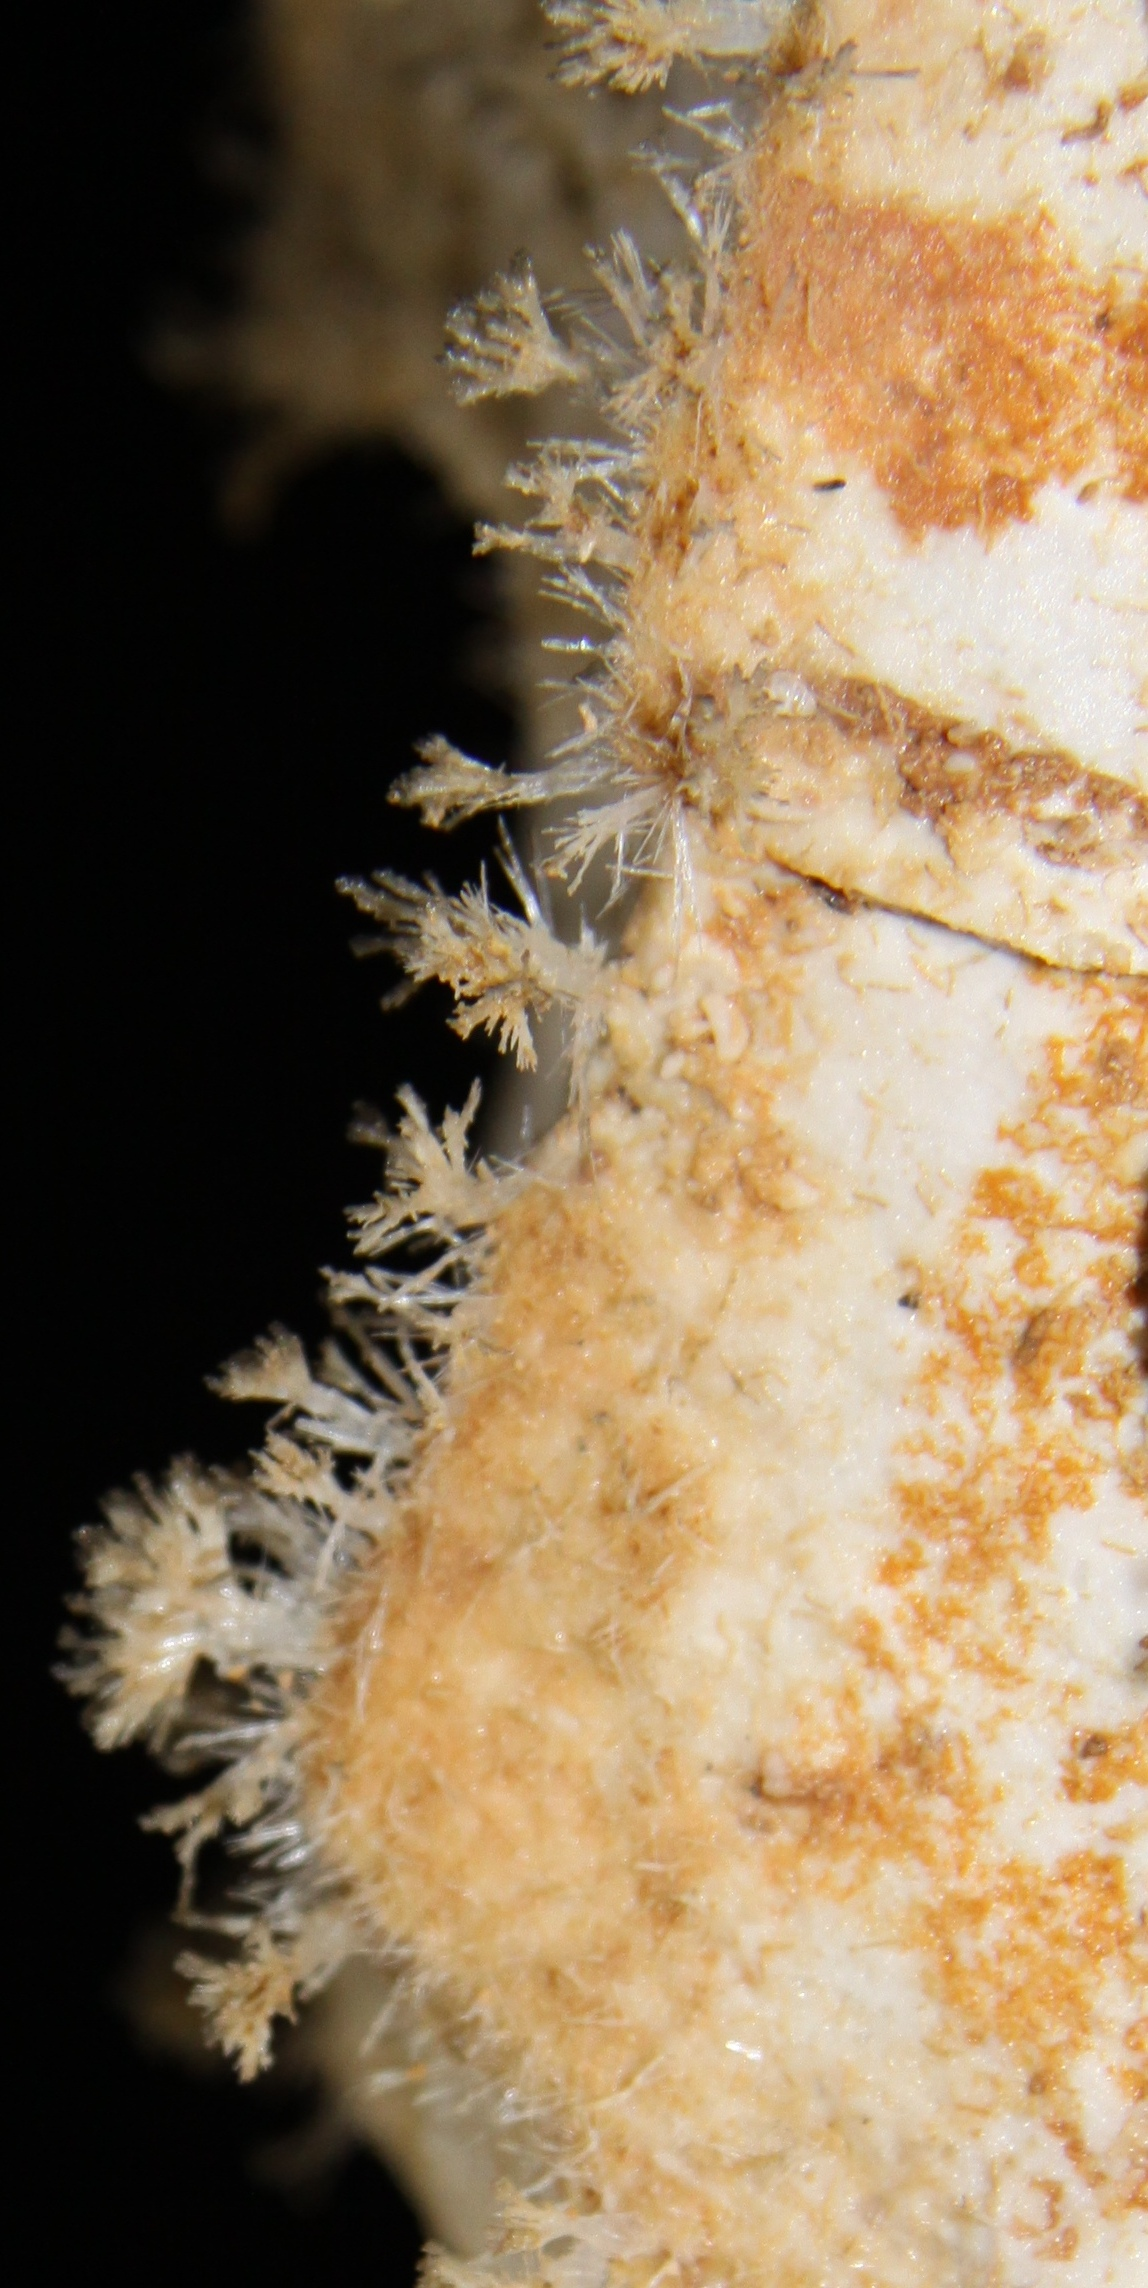
\includegraphics[width=\linewidth]{2010/expo_findings/20100731-19-03-16 - Martin McGowan Canon 50D - IMG_1488 - Delicate Crystals at start of Palace of King Minos--orig.jpg}} 
\caption{Crystal formations at the start of the \protect\passage{Palace of King Minos}. \pic{Martin McGowan}} \label{Minos crystals 1}
\end{marginfigure}

\passage{Leopard} became the great focus of exploration this year, leading to 1.5 km of new
passage. This lead (a window off \passage{Zimmer} chamber, now a 15 m `up' pitch) had also been originally discovered in 2001, but the drop that it led to had lain untouched since then.

This was partially due to its loose and muddy nature, but also that deep
exploration had concentrated on good leads elsewhere (most particularly
the lower \passage{Vrtnarija} level accessed with the bottoming of
\passage{Big Rock}). This pitch took several sessions of rigging and
gardening to successfully conquer, and is now named \passage{Cheetah} (P35
m), because of the sense of having cheated death that it engenders on
passing\sidenote{As with other loose pitches, this stabilised considerably over
the next few years.}. There are several windows off \passage{Cheetah},
which are definitely promising\sidenote{One was revisited by Jan and Kate in 2011, and found to be an alcove.},
although not easily accessible because of the broken nature of the rock.

At the bottom, this pitch intersects a horizontal fossil passage, which can be divided into three main horizontal areas:

\textbf{\passage{Wonderland}} (heading South) linking into \passage{Rolling Stones},
\passage{Hidden Surprise}, \passage{Mudstone Traverse}, \passage{Kamikaze} and
finally \passage{Lost Hopes}. This is mainly dry with large breakdown
chambers.

\textbf{\passage{Prince Consort Road}} (heading North) was initially pushed to the \passage{Albert Hall} (from where the \passage{Serpentine} meander leads off to the \passage{It Will Rain for a Million Years} pitch). This passage bisects three streamways (one of which was pushed and forms the \passage{Esoterica} series) and includes considerable calcite formations.

From the \passage{Albert Hall} a climb was made into the \textbf{\passage{Palace of King Minos}}. This passage is complex, and side branches have neither
been fully explored nor surveyed. The known passage leads via \passage{Minotaur Rift} to terminate in the \passage{Queen's Bedchamber} where the draught disappears towards the ceiling.

Together this passage leading off from \passage{Cheetah} has been explored to over 1.5 km in length, and we are sure that more is yet to be found.

A significant volume of air flows through these regions, indicating that there may be further developments.


\subsection{Wonderland}

\passage{Wonderland} is the southern-most of the horizontal development,
leading directly off from \passage{Cheetah}. It was pushed to a small pitch
dropping into a boulder filled chamber, \passage{Rolling Stones}, which was
the limit of the first exploration trip due to the lack of rope. This
chamber is situated right below \passage{Zimmer}, about 40 m deeper. There is a
further, as yet unpushed, pitch going down between the large, seemingly unstable, boulders on the floor.

A happenstance crawl behind some boulders led to further drafting
passage (\passage{Hidden Surprise}), which, after traversing another
chamber and crawl, finishes in a chamber with a massive hole in the
floor (\passage{Kamikaze} pitch). The passage continues on the far side of
the pitch (traversed on mud along the left wall); however, due to the
collapsed ceiling, these developments are almost two-dimensional
(\passage{Mudstone Squeeze}). The squeeze, which is filled with interesting
fossilised mud formations, was pushed to the limits of comfort, although
\bignote{it still continues}.

\passage{Kamikaze} consists of a series of small ledges. From the second
ledge a tell tale breeze led to an interesting bedding plane crawl
pushed upwind but still untouched downwind. The pitch was bottomed (\passage{Lost
Hopes}), wherein an inlet was followed down a 10 m pitch to a series of
squeezes and rifts which quickly became tight. There is a ledge halfway
down \passage{Lost Hopes}, with a perhaps larger abandoned rift.

These three leads (\passage{Kamikaze}, \passage{Mudstone}, \passage{Lost Hopes}) are of
interest as they now form the most Easterly extent of \passage{Vrtnarija}
at depth, seeming to `spear' through the large N-S geological feature
that contains the majority of the horizontal passage.

The whole area of \passage{Wonderland} is extremely dry, quiet and rather
spacious in its scope. It is particularly \bignote{reminiscent of the higher
level passage in the \passage{Easegill} system, Yorkshire}.


\subsection{Prince Consort Road}

\passage{Prince Consort Road} is the passage going north from
\passage{Cheetah}. Several small streams intersect it and some formations
have been found. The discovery of stalactites covered with helictites
proved particularly exciting! The passage leads to a small boulder choke
which was easily passed and led to a large chamber (the \passage{Albert Hall}).

Before the \passage{Albert Hall}, three apparently unique streamways have been found:


\begin{pagefigure}
\checkoddpage \ifoddpage \forcerectofloat \else \forceversofloat \fi
   \centering
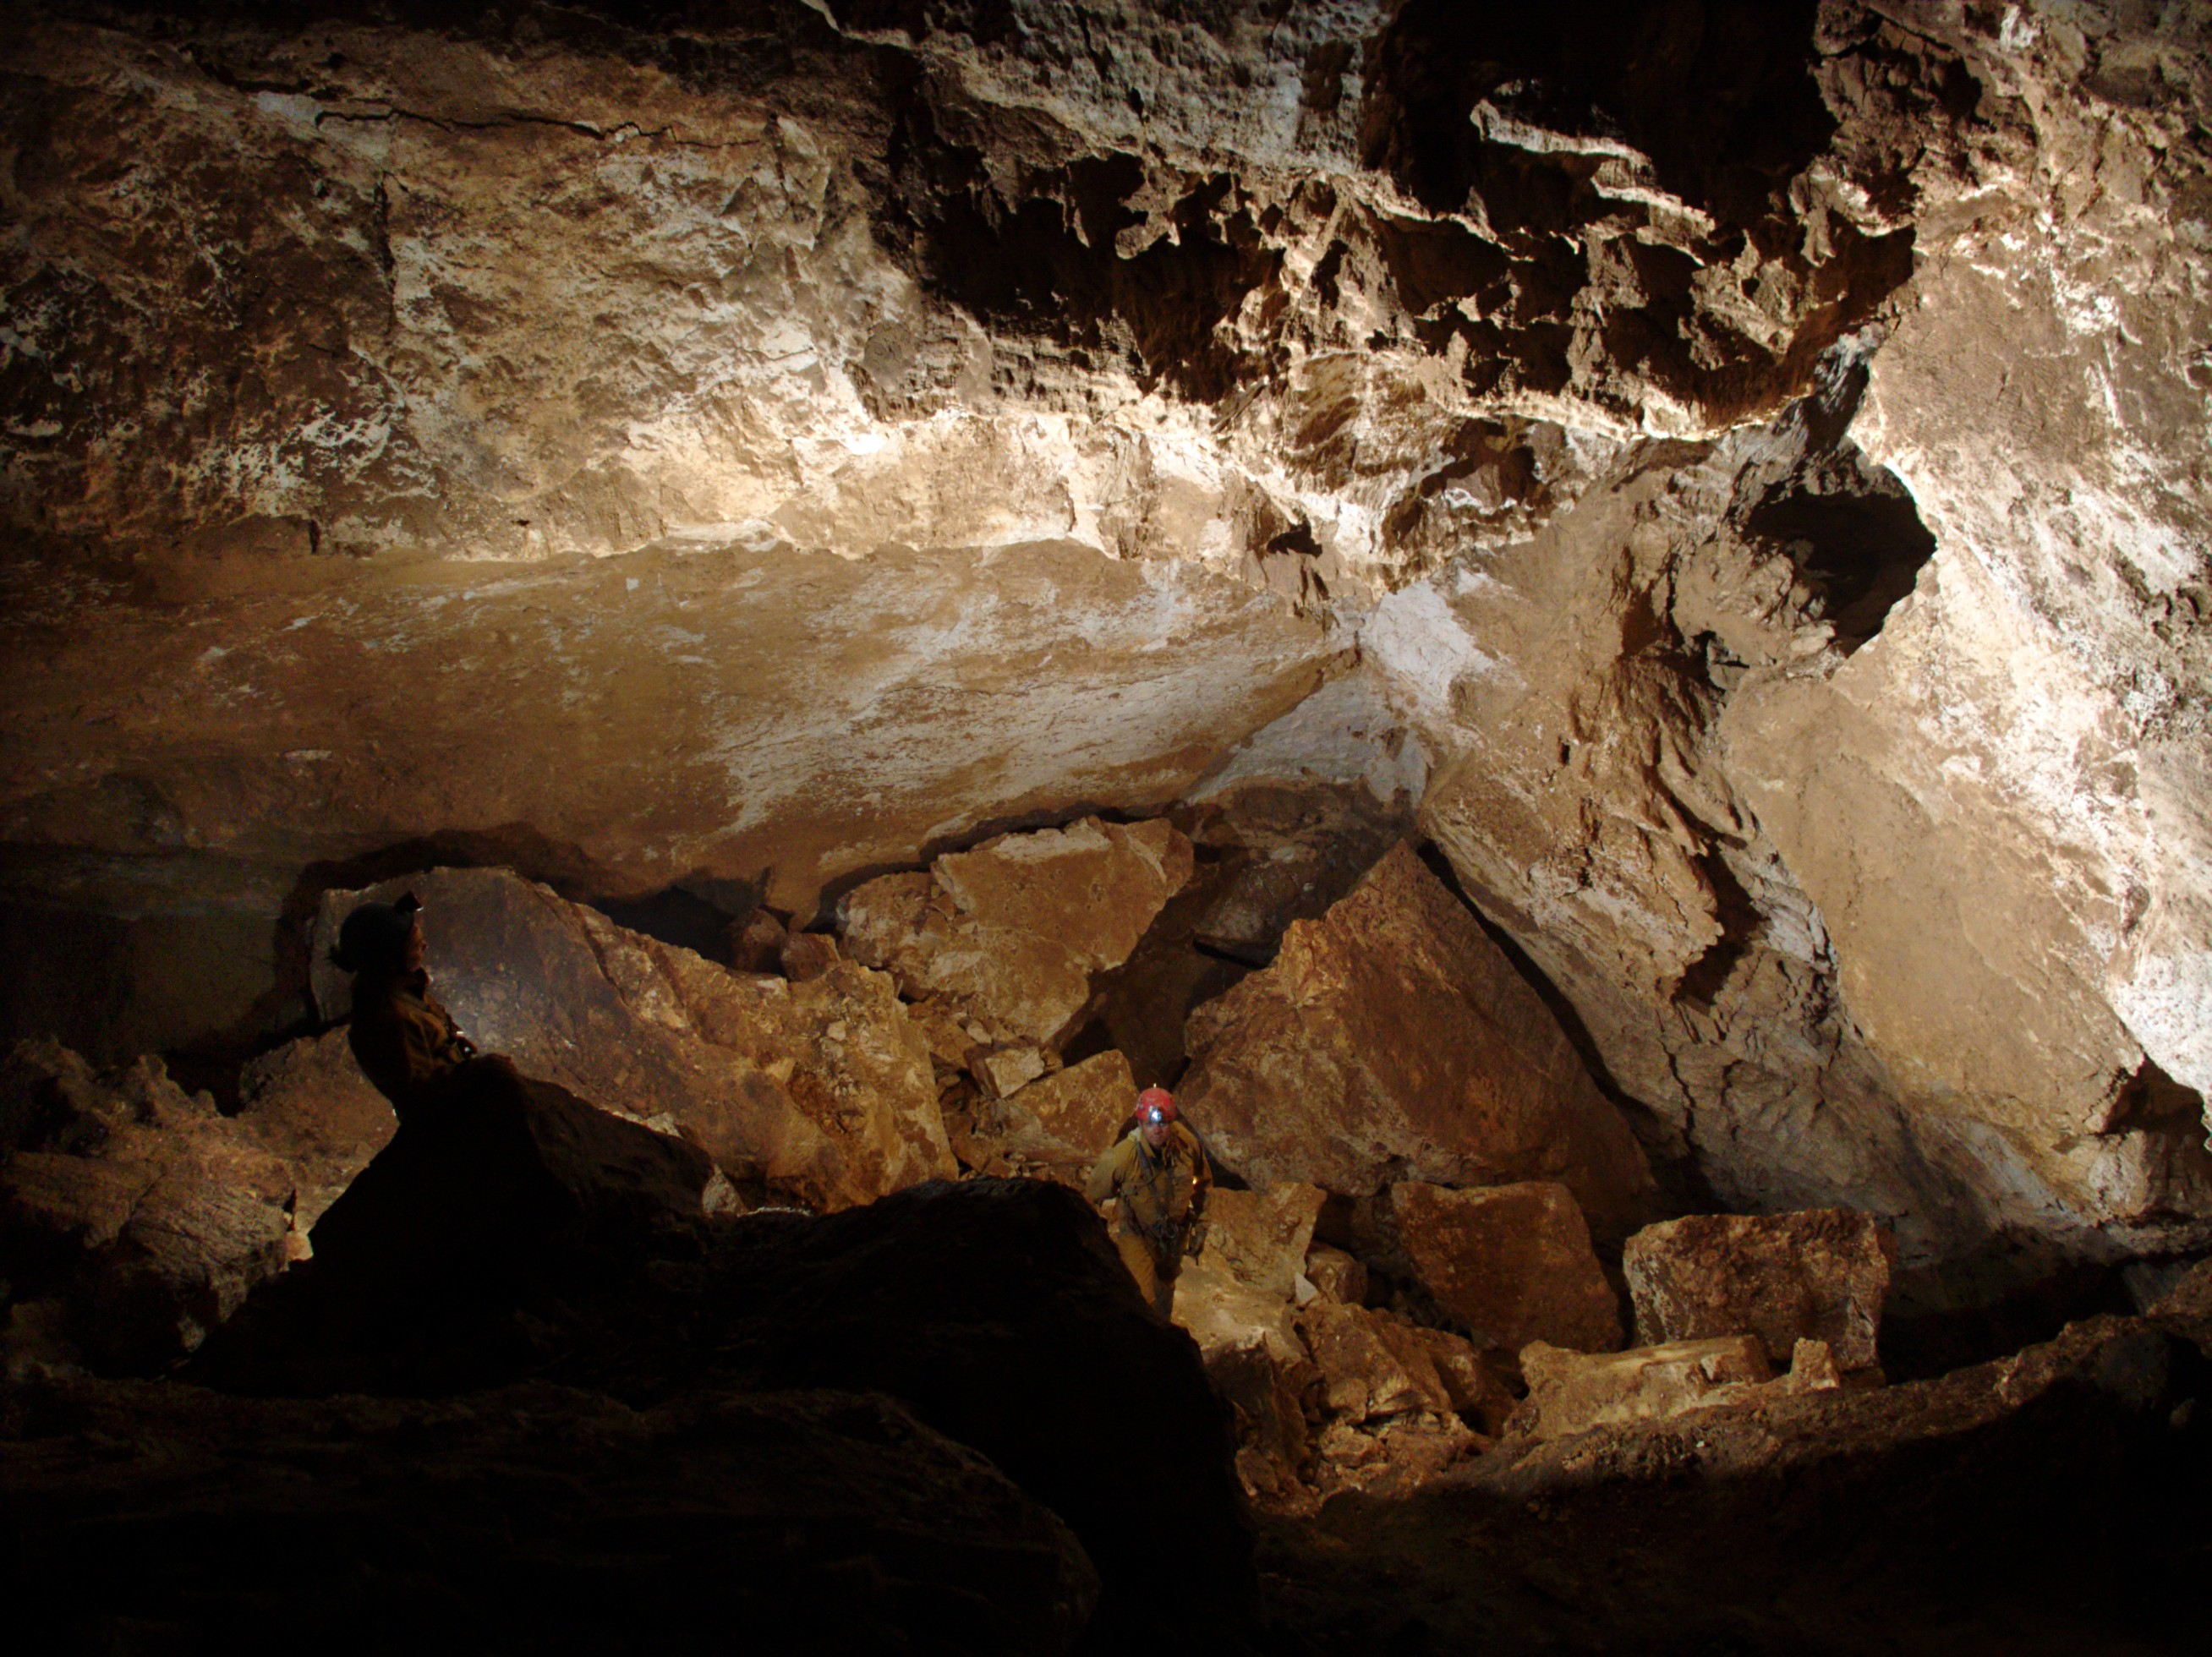
\includegraphics[width = \textwidth]{2010/expo_findings/20100731-21-53-00-Jarvist Frost-Canon G5-CRW_0402-Albert Hall - Prince Consort Road--orig.jpg}
\caption{Tim Wright, aka Shed, in the \protect\passage{Albert Hall}. \pic{Jarvist Frost}} \label{Albert Hall}
\end{pagefigure}


One intersecting the passage along a traverse (water chokes into boulder floor), then around a small chamber at about halfway to \passage{Albert Hall}, on a corner of the main passage approximately 2/3 of the way to
the \passage{Albert Hall} a small rift to the east, and a nice white-sanded water inlet to the west. The latter leads to an unpushed pitch under the main passage -- there is a cairn and note mentioning the lead. Of these,
only the second has been pushed, into the \passage{Esoterica} series. Strangely this wet, tight rift has only been visited once during the
expedition, even though it is still going.

In the \passage{Albert Hall} two streams enter the chamber from on high
(the ceiling was measured as being over 30 m up, by laser disto) and join into a rather beautiful spacious vadose streamway (the \passage{Serpentine}).
\passage{Serpentine} was pushed and leads to another split pitch (\passage{It Will Rain for a Million Years} -- pushed during a continuing flood pulse).
At the bottom of \passage{It Will Rain} pitch the stream continues and has not been explored.


\subsection{The Palace of King Minos}

North from the \passage{Albert Hall} a muddy climb lead to \passage{The Palace of King Minos}. This passage and its continuation (the \passage{Minotaur Rift}) has some of the most beautiful formations found on \passage{Migovec} to date, in particular fine walls of calcite, gypsum and aragonite crystals, mud formations and weird soot encrusted floors. The \passage{Palace of King Minos} has a labyrinthine nature with several passages leading back to \passage{Albert Hall}, the largest loop of which was named \passage{Ouroboros}.

The passage has a classic large phreatic lozenge shape, with some parts undercut by fossil vadose passage. Near the start of the passage a
significant breeze blew through a small hole. This was enlarged and found to lead to a small phreatic tube which bizarrely led into an active vadose streamway (\passage{Povodni Mož} -- Water Nymph). \passage{Povodni Mož} has been pushed upstream to a large active aven (and smaller dry parallel shaft), and downstream to a sump (approximately 2mx2 m in size in the corner of a small chamber and taking the small flow) and has hence been derigged.


    \begin{marginfigure}
\checkoddpage \ifoddpage \forcerectofloat \else \forceversofloat \fi
\centering
 \frame{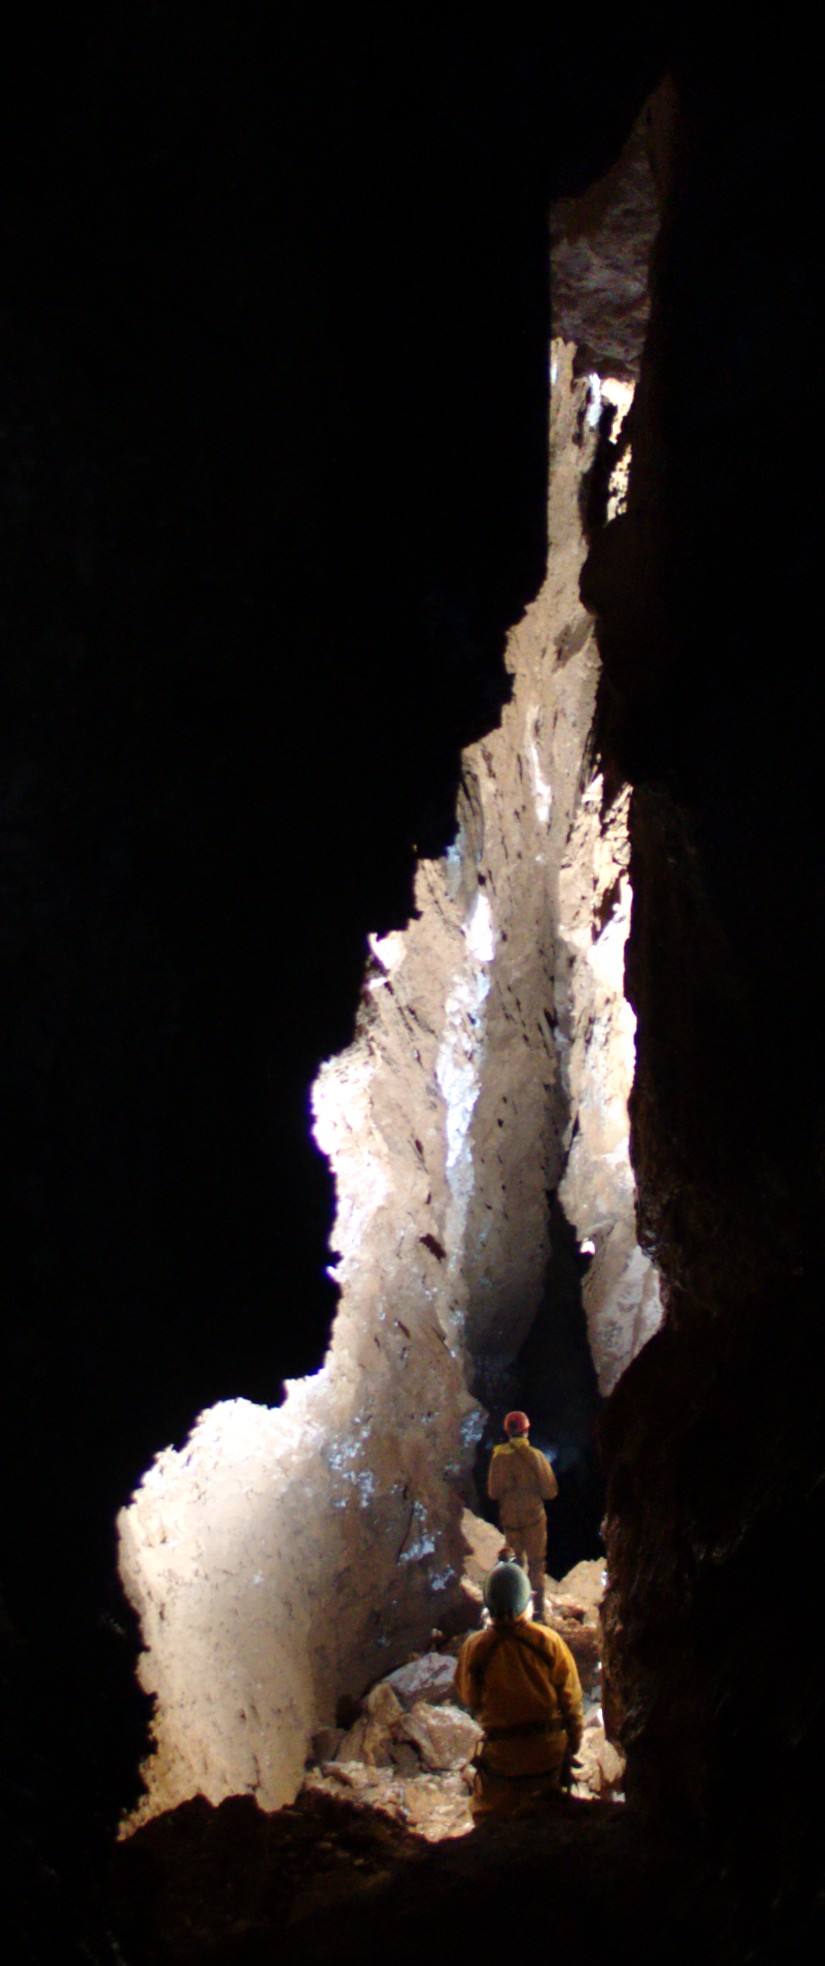
\includegraphics[width=\linewidth]{2010/expo_findings/20100731-19-46-56-Jarvist Frost-Canon G5-CRW_0338-crop-Minotaur Rift - Palace of King Minos--orig.jpg}} 
 \caption{The \protect\passage{Minotaur Rift}. \pic{Jarvist Frost}}
 \label{minotaur rift 2010}
\end{marginfigure}

Continuing along the main \passage{Palace} passage several horizontal tubes have been explored which lead back into the main passage, though not all have
been entered in the survey. Eventually the main route leads to a high and wide rift (\passage{Minotaur Rift} -- 20 m high, 60 m long) beyond
which the best formations are to be found. This passage has a few interesting leads in it: a high, dry, circular, muddy window to the right of the passage near a tiny inlet, 2 small tubes leading off the main passage which both need a little mechanical persuasion.

The chambers beyond \passage{Minotaur Rift} are spacious and display massive amounts of crystal formation on all available surfaces -- there is
white `popcorning' almost everywhere, with regions of more intricate needle and feather formations. The chambers decay into a crawl, which almost unbelievably is over a smooth calcite floor. This leads to a classic boulder choke gallery (choking at the end). On the left a small boulder choke climb leads to the \passage{Queen's Bedchamber}. In this large room, the draught appears to disappear up towards the ceiling -- both ends of
the chamber are potential climbing projects ($\approx$ +20 m).

The region is extremely reminiscent of \passage{Ogof Ffynnon Ddu II} in Wales.


\subsection{Tolminska Korita}

This lead off \passage{Zimmer} chamber had been discovered in 2001 but had lain unexplored until last year, when the first few pits of the active meander were pushed to a larger pitch. \passage{Tolminska Korita} developed into cascades of active pitches (\passage{Black Knight} series) to a duck. The
duck was soon bypassed by a 5 m free climb into old phreatic level.

The passage beyond soon diverges into two continuations:



    \begin{marginfigure}
\checkoddpage \ifoddpage \forcerectofloat \else \forceversofloat \fi
\centering
 \frame{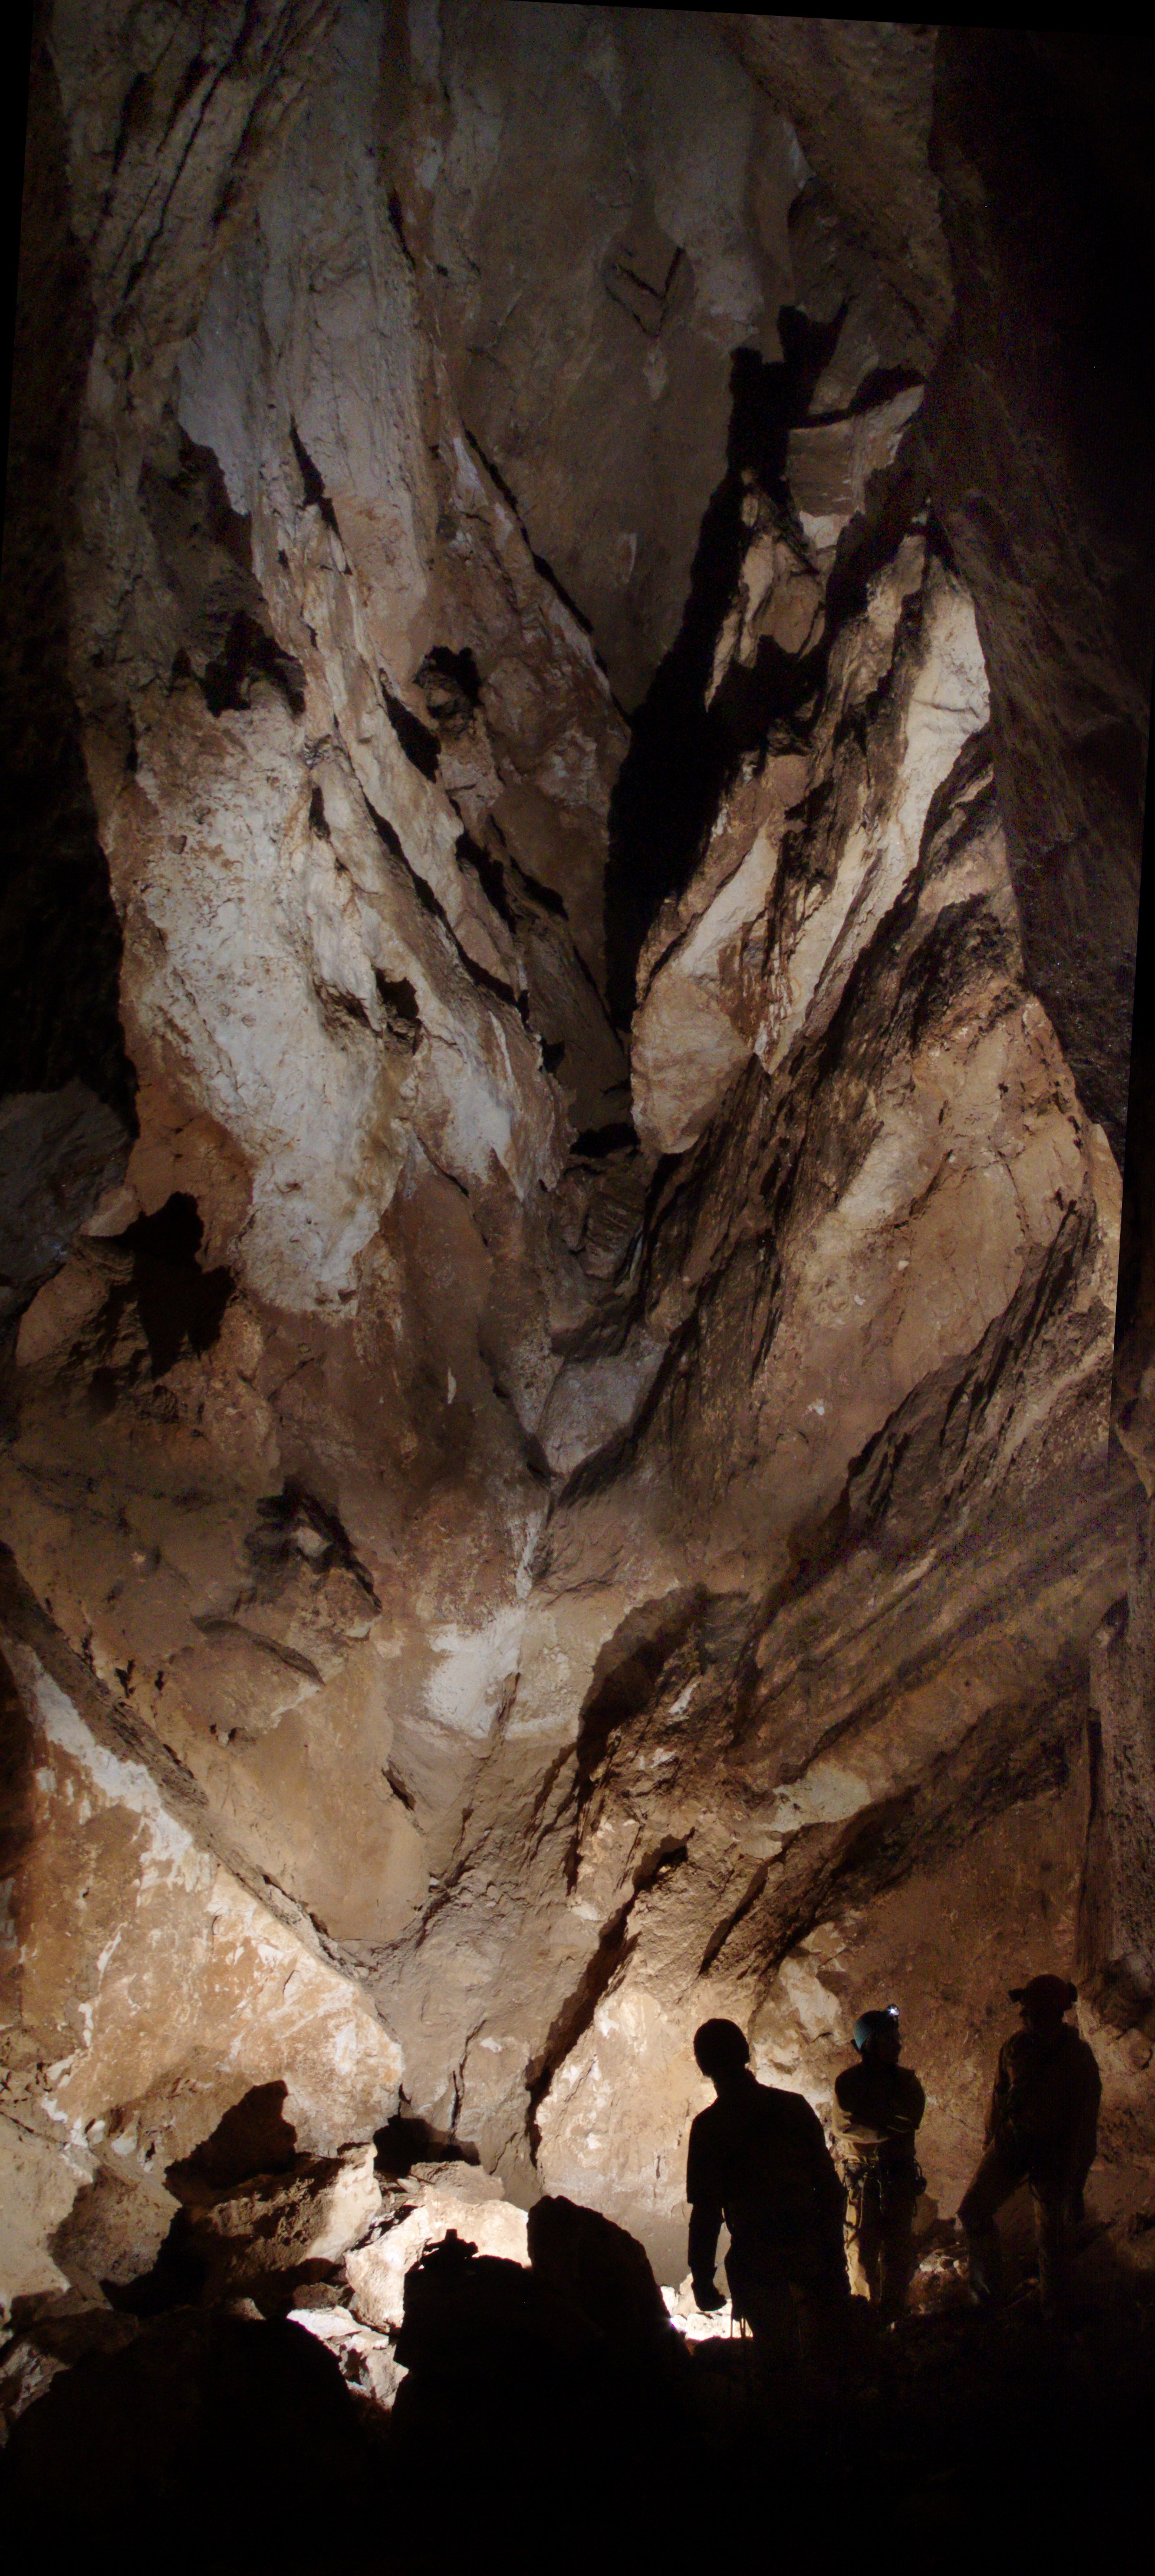
\includegraphics[width=\linewidth]{2010/expo_findings/20100731-20-41-52-Jarvist Frost-Canon G5-CRW_0368-montage-Queens Bed Chamber - Palace of King Minos--orig.jpg}} 
 \caption{A composite photograph of the \protect\passage{Queen's Bedchamber}. \pic{Jarvist Frost}}
 \label{qbc}
\end{marginfigure}

\subsection{\passage{Sidewinder}, \passage{Crack in
Time}}

The higher dust-filled dry phreatic level (\passage{Sidewinder}, \passage{Crack in Time}) connects into \passage{Envy} in the low level via
free climbs and two small pitches. It is not particularly surprising that the \passage{Crack in Time} was not explored from below, as the
connection is made by a long body-sized crawl above a thin (5 cm) crack connecting to known passage (\passage{Envy}), which happily pops out at the
top of a obscure 3 m free climb. Connecting into a 2004-era permanent survey station, \passage{Korita} now forms a second loop in \passage{Vrtnarija},
forming \passage{Vrtnarija} into a figure-8 shape with \passage{Friendship Gallery} at the waist.

\subsection{\passage{White Bishop}, \passage{Stalemate}}

The active streamway descends two 10-15 m pitches connected with a spacious meander incorporating free climbable cascades, before ending in an impassable rift (-662 m).

This water disappears into `blank mountain' on our survey, but would require considerable effort to progress, and \passage{Korita} was thus derigged.


\subsection{\passage{Roaring} (\passage{Muddy
Window} off \passage{Happy Monday})}

This was regained by bolt climbing from the bottom of \passage{Happy Monday} to regain the \passage{Muddy Window}.

The climb in the mud chamber was made, but quickly led to a large boulder blocking the way (\passage{Roaring}). A tight rift taking a large draught was left unpushed. Progress is believed to require expansion\sidenote{of the chemical kind}.

\subsection{\passage{Friendship Gallery} Leads}

Similarly the traverse to an inlet on \passage{Falls Road}, and the continuation of \passage{Falls Road} itself was left unpushed. A small dig was made in \passage{Friendship Gallery} beyond \passage{Prima Junction}, which led to a small unpushed pitch above a stream.

\subsection{Deep Leads Below \passage{Big Rock Candy
Mountain}}

\subsection{\passage{Insomnia} - \passage{Republika}
Streamway}

Last year a `written off' streamway \passage{Republika}, leading from
\passage{Red Cow}) was found and pushed upstream to an aven-fed watershed, then down the other limb to a rift pitch.

With the promise of being one of the deepest points of the cave a return in 2010 was obligatory. The pitch was found to be 41 m and was pushed down a continuing active rift (\passage{Insomnia}). The end is now only 4 m higher than \passage{Colorado Sump} (the deepest known point of \passage{Vrtnarija}).
Since the limit of exploration is above a small 4-5 m pitch it is understood that in 2011 this will inevitably become the deepest passage
in the system, and the signs are good for continuing development of depth. The end is 802 m below the entrance of \passage{Vrtnarija}, but the
\passage{M2} (\passage{Kavkna Jama}) entrance is 75 m higher still, and a connection between the systems would make this point -877 m deep overall, with
potential for further depth extension.

\begin{marginfigure}
\checkoddpage \ifoddpage \forcerectofloat \else \forceversofloat \fi
   \centering
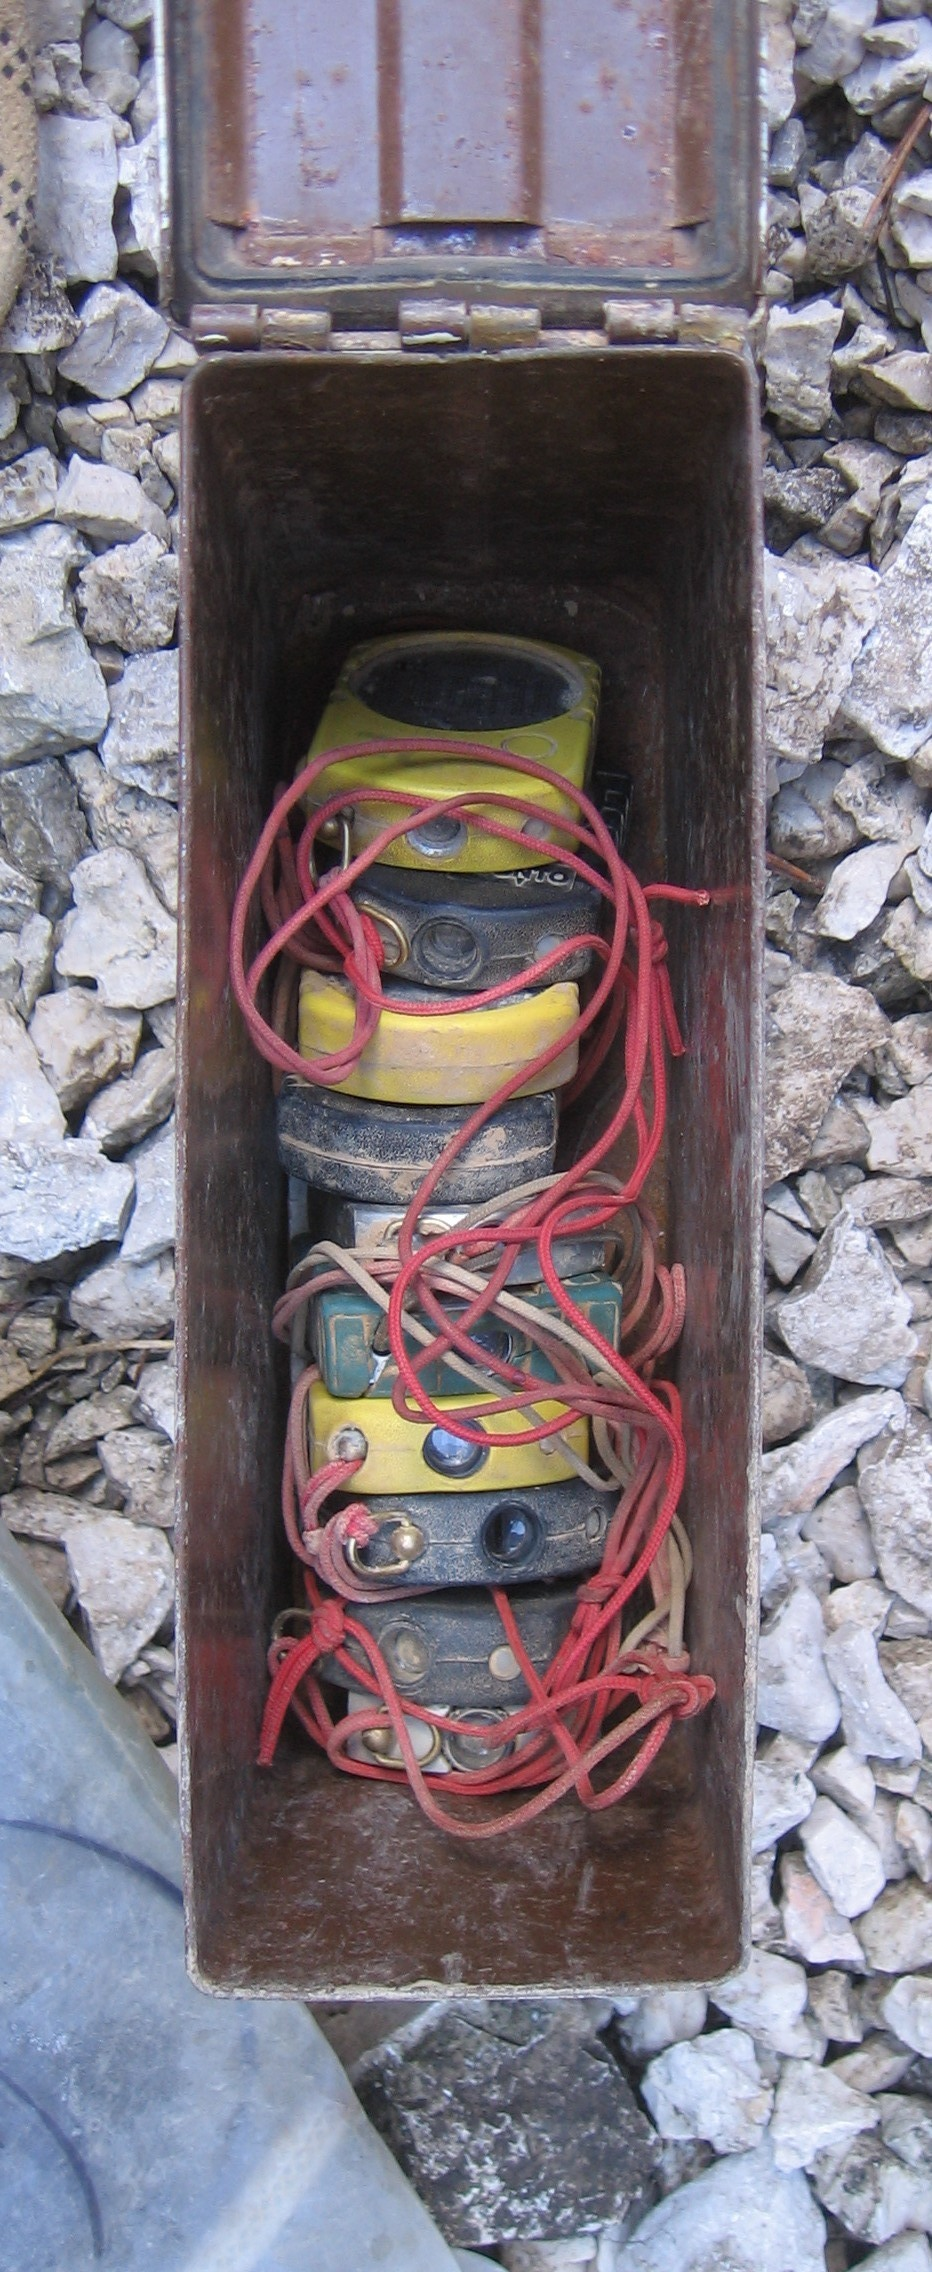
\includegraphics[width = \textwidth]{2010/expo_findings/20100811-12-17-38 - Jarvist Frost A520 - IMG_0041 - survey instruments.jpg}
\caption{Survey instruments collected together at the end of expo. \pic{Jarvist Frost}} \label{ammo tin instruments}
\end{marginfigure}

\subsection{\passage{Balamory}}

A return to \passage{Balamory} was thwarted by lack of rope of the exploratory party (one more pitch than expected on route), but the team made good use of the trip to the depths by recovering the camping mats from the deep 2004 camp (\passage{The Fridge}, near \passage{Cactus Junction}), and prospecting for other leads with some success.

\subsection{October 2010 -- M2 (Kavkna Jama)}

The JSPDT organised a trip based at the mountain hut at \passage{Kal} on 2nd
October 2010. The terminal rift was enlarged to gain a
\textasciitilde 20 m pitch and a larger, undescended (due to lack of rope), pitch.

A return trip three weeks later descended the pitch and found it to be
\(\approx\) 60 m. The cave closes immediately, with a tight rift taking
the water and a slightly larger abandoned rift also offering potential.
It draughts strongly.

The \passage{M2} cavers returned in thick fog, following their footsteps
through the 10 cm deep snow. With the coming winter Migovec is
effectively closed for exploration until summer 2011.



